\documentclass[11pt,compress,t,notes=noshow, xcolor=table]{beamer}
\usepackage[]{graphicx}\usepackage[]{color}
% maxwidth is the original width if it is less than linewidth
% otherwise use linewidth (to make sure the graphics do not exceed the margin)
\makeatletter
\def\maxwidth{ %
  \ifdim\Gin@nat@width>\linewidth
    \linewidth
  \else
    \Gin@nat@width
  \fi
}
\makeatother

\definecolor{fgcolor}{rgb}{0.345, 0.345, 0.345}
\newcommand{\hlnum}[1]{\textcolor[rgb]{0.686,0.059,0.569}{#1}}%
\newcommand{\hlstr}[1]{\textcolor[rgb]{0.192,0.494,0.8}{#1}}%
\newcommand{\hlcom}[1]{\textcolor[rgb]{0.678,0.584,0.686}{\textit{#1}}}%
\newcommand{\hlopt}[1]{\textcolor[rgb]{0,0,0}{#1}}%
\newcommand{\hlstd}[1]{\textcolor[rgb]{0.345,0.345,0.345}{#1}}%
\newcommand{\hlkwa}[1]{\textcolor[rgb]{0.161,0.373,0.58}{\textbf{#1}}}%
\newcommand{\hlkwb}[1]{\textcolor[rgb]{0.69,0.353,0.396}{#1}}%
\newcommand{\hlkwc}[1]{\textcolor[rgb]{0.333,0.667,0.333}{#1}}%
\newcommand{\hlkwd}[1]{\textcolor[rgb]{0.737,0.353,0.396}{\textbf{#1}}}%
\let\hlipl\hlkwb

\usepackage{framed}
\makeatletter
\newenvironment{kframe}{%
 \def\at@end@of@kframe{}%
 \ifinner\ifhmode%
  \def\at@end@of@kframe{\end{minipage}}%
  \begin{minipage}{\columnwidth}%
 \fi\fi%
 \def\FrameCommand##1{\hskip\@totalleftmargin \hskip-\fboxsep
 \colorbox{shadecolor}{##1}\hskip-\fboxsep
     % There is no \\@totalrightmargin, so:
     \hskip-\linewidth \hskip-\@totalleftmargin \hskip\columnwidth}%
 \MakeFramed {\advance\hsize-\width
   \@totalleftmargin\z@ \linewidth\hsize
   \@setminipage}}%
 {\par\unskip\endMakeFramed%
 \at@end@of@kframe}
\makeatother

\definecolor{shadecolor}{rgb}{.97, .97, .97}
\definecolor{messagecolor}{rgb}{0, 0, 0}
\definecolor{warningcolor}{rgb}{1, 0, 1}
\definecolor{errorcolor}{rgb}{1, 0, 0}
\newenvironment{knitrout}{}{} % an empty environment to be redefined in TeX

\usepackage{alltt}
\newcommand{\SweaveOpts}[1]{}  % do not interfere with LaTeX
\newcommand{\SweaveInput}[1]{} % because they are not real TeX commands
\newcommand{\Sexpr}[1]{}       % will only be parsed by R
\newcommand{\xmark}{\ding{55}}%


\usepackage[english]{babel}
\usepackage[utf8]{inputenc}

\usepackage{dsfont}
\usepackage{verbatim}
\usepackage{amsmath}
\usepackage{amsfonts}
\usepackage{amssymb}
\usepackage{bm}
\usepackage{csquotes}
\usepackage{multirow}
\usepackage{longtable}
\usepackage{booktabs}
\usepackage{enumerate}
\usepackage[absolute,overlay]{textpos}
\usepackage{psfrag}
\usepackage{algorithm}
\usepackage{algpseudocode}
\usepackage{eqnarray}
\usepackage{arydshln}
\usepackage{tabularx}
\usepackage{placeins}
\usepackage{tikz}
\usepackage{setspace}
\usepackage{colortbl}
\usepackage{mathtools}
\usepackage{wrapfig}
\usepackage{bm}
\usepackage{amsmath}
\usepackage{pifont}
\usepackage[round]{natbib}
\usepackage{hyperref}

\usetikzlibrary{shapes,arrows,automata,positioning,calc,chains,trees, shadows}
\tikzset{
  %Define standard arrow tip
  >=stealth',
  %Define style for boxes
  punkt/.style={
    rectangle,
    rounded corners,
    draw=black, very thick,
    text width=6.5em,
    minimum height=2em,
    text centered},
  % Define arrow style
  pil/.style={
    ->,
    thick,
    shorten <=2pt,
    shorten >=2pt,}
}

\usepackage{subfig}

% Defines macros and environments
\usepackage{../../style/lmu-lecture}


\let\code=\texttt
\let\proglang=\textsf

\setkeys{Gin}{width=0.9\textwidth}

\setbeamertemplate{frametitle}{\expandafter\uppercase\expandafter\insertframetitle}

% basic latex stuff
\newcommand{\pkg}[1]{{\fontseries{b}\selectfont #1}} % fontstyle for R packages

% Often used in exercise Rnw files, still relevant?
\newcommand{\lz}{\vspace{0.5cm}} % vertical space
\newcommand{\dlz}{\vspace{1cm}}  % double vertical space

% Unused and about to be deleted
\newcommand{\oneliner}[1] % Oneliner for important statements
{\begin{block}{}\begin{center}\begin{Large}#1\end{Large}\end{center}\end{block}}


%--------------------%
%  New environments  %
%--------------------%

 % Frame with breaks and verbatim // this is used very often
\newenvironment{vbframe}
{
\begin{frame}[containsverbatim,allowframebreaks]
}
{
\end{frame}
}

% Frame with verbatim without breaks (to avoid numbering one slided frames)
% This is not used anywhere but I can see it being useful
\newenvironment{vframe}
{
\begin{frame}[containsverbatim]
}
{
\end{frame}
}

% Itemize block
\newenvironment{blocki}[1]
{
\begin{block}{#1}\begin{itemize}
}
{
\end{itemize}\end{block}
}

%--------------%
%  Citebutton  %
%--------------%
% Example usage (from slides-cart-discussion.tex)
% \citebutton{Breiman, 1984}{https://www.taylorfrancis.com/books/mono/10.1201/9781315139470/classification-regression-trees-leo-breiman}
\newcommand{\citebutton}[2]{%
\NoCaseChange{\resizebox{!}{9pt}{\protect\beamergotobutton{\href{#2}{#1}}}}%
}

% textcolor that works in mathmode
% https://tex.stackexchange.com/a/261480
% Used e.g. in forests/slides-forests-bagging.tex
% [...] \textcolor{blue}{\tfrac{1}{M}\sum^M_{m} [...]
\makeatletter
\renewcommand*{\@textcolor}[3]{%
  \protect\leavevmode
  \begingroup
    \color#1{#2}#3%
  \endgroup
}
\makeatother





% dependencies: amsmath, amssymb, dsfont
% math spaces
\ifdefined\N
\renewcommand{\N}{\mathds{N}} % N, naturals
\else \newcommand{\N}{\mathds{N}} \fi
\newcommand{\Z}{\mathds{Z}} % Z, integers
\newcommand{\Q}{\mathds{Q}} % Q, rationals
\newcommand{\R}{\mathds{R}} % R, reals
\ifdefined\C
\renewcommand{\C}{\mathds{C}} % C, complex
\else \newcommand{\C}{\mathds{C}} \fi
\newcommand{\continuous}{\mathcal{C}} % C, space of continuous functions
\newcommand{\M}{\mathcal{M}} % machine numbers
\newcommand{\epsm}{\epsilon_m} % maximum error

% counting / finite sets
\newcommand{\setzo}{\{0, 1\}} % set 0, 1
\newcommand{\setmp}{\{-1, +1\}} % set -1, 1
\newcommand{\unitint}{[0, 1]} % unit interval

% basic math stuff
\newcommand{\xt}{\tilde x} % x tilde
\DeclareMathOperator*{\argmax}{arg\,max} % argmax
\DeclareMathOperator*{\argmin}{arg\,min} % argmin
\newcommand{\argminlim}{\mathop{\mathrm{arg\,min}}\limits} % argmax with limits
\newcommand{\argmaxlim}{\mathop{\mathrm{arg\,max}}\limits} % argmin with limits
\newcommand{\sign}{\operatorname{sign}} % sign, signum
\newcommand{\I}{\mathbb{I}} % I, indicator
\newcommand{\order}{\mathcal{O}} % O, order
\newcommand{\bigO}{\mathcal{O}} % Big-O Landau
\newcommand{\littleo}{{o}} % Little-o Landau
\newcommand{\pd}[2]{\frac{\partial{#1}}{\partial #2}} % partial derivative
\newcommand{\floorlr}[1]{\left\lfloor #1 \right\rfloor} % floor
\newcommand{\ceillr}[1]{\left\lceil #1 \right\rceil} % ceiling
\newcommand{\indep}{\perp \!\!\! \perp} % independence symbol

% sums and products
\newcommand{\sumin}{\sum\limits_{i=1}^n} % summation from i=1 to n
\newcommand{\sumim}{\sum\limits_{i=1}^m} % summation from i=1 to m
\newcommand{\sumjn}{\sum\limits_{j=1}^n} % summation from j=1 to p
\newcommand{\sumjp}{\sum\limits_{j=1}^p} % summation from j=1 to p
\newcommand{\sumik}{\sum\limits_{i=1}^k} % summation from i=1 to k
\newcommand{\sumkg}{\sum\limits_{k=1}^g} % summation from k=1 to g
\newcommand{\sumjg}{\sum\limits_{j=1}^g} % summation from j=1 to g
\newcommand{\meanin}{\frac{1}{n} \sum\limits_{i=1}^n} % mean from i=1 to n
\newcommand{\meanim}{\frac{1}{m} \sum\limits_{i=1}^m} % mean from i=1 to n
\newcommand{\meankg}{\frac{1}{g} \sum\limits_{k=1}^g} % mean from k=1 to g
\newcommand{\prodin}{\prod\limits_{i=1}^n} % product from i=1 to n
\newcommand{\prodkg}{\prod\limits_{k=1}^g} % product from k=1 to g
\newcommand{\prodjp}{\prod\limits_{j=1}^p} % product from j=1 to p

% linear algebra
\newcommand{\one}{\bm{1}} % 1, unitvector
\newcommand{\zero}{\mathbf{0}} % 0-vector
\newcommand{\id}{\bm{I}} % I, identity
\newcommand{\diag}{\operatorname{diag}} % diag, diagonal
\newcommand{\trace}{\operatorname{tr}} % tr, trace
\newcommand{\spn}{\operatorname{span}} % span
\newcommand{\scp}[2]{\left\langle #1, #2 \right\rangle} % <.,.>, scalarproduct
\newcommand{\mat}[1]{\begin{pmatrix} #1 \end{pmatrix}} % short pmatrix command
\newcommand{\Amat}{\mathbf{A}} % matrix A
\newcommand{\Deltab}{\mathbf{\Delta}} % error term for vectors

% basic probability + stats
\renewcommand{\P}{\mathds{P}} % P, probability
\newcommand{\E}{\mathds{E}} % E, expectation
\newcommand{\var}{\mathsf{Var}} % Var, variance
\newcommand{\cov}{\mathsf{Cov}} % Cov, covariance
\newcommand{\corr}{\mathsf{Corr}} % Corr, correlation
\newcommand{\normal}{\mathcal{N}} % N of the normal distribution
\newcommand{\iid}{\overset{i.i.d}{\sim}} % dist with i.i.d superscript
\newcommand{\distas}[1]{\overset{#1}{\sim}} % ... is distributed as ...

% machine learning
\newcommand{\Xspace}{\mathcal{X}} % X, input space
\newcommand{\Yspace}{\mathcal{Y}} % Y, output space
\newcommand{\Zspace}{\mathcal{Z}} % Z, space of sampled datapoints
\newcommand{\nset}{\{1, \ldots, n\}} % set from 1 to n
\newcommand{\pset}{\{1, \ldots, p\}} % set from 1 to p
\newcommand{\gset}{\{1, \ldots, g\}} % set from 1 to g
\newcommand{\Pxy}{\mathbb{P}_{xy}} % P_xy
\newcommand{\Exy}{\mathbb{E}_{xy}} % E_xy: Expectation over random variables xy
\newcommand{\xv}{\mathbf{x}} % vector x (bold)
\newcommand{\xtil}{\tilde{\mathbf{x}}} % vector x-tilde (bold)
\newcommand{\yv}{\mathbf{y}} % vector y (bold)
\newcommand{\xy}{(\xv, y)} % observation (x, y)
\newcommand{\xvec}{\left(x_1, \ldots, x_p\right)^\top} % (x1, ..., xp)
\newcommand{\Xmat}{\mathbf{X}} % Design matrix
\newcommand{\allDatasets}{\mathds{D}} % The set of all datasets
\newcommand{\allDatasetsn}{\mathds{D}_n}  % The set of all datasets of size n
\newcommand{\D}{\mathcal{D}} % D, data
\newcommand{\Dn}{\D_n} % D_n, data of size n
\newcommand{\Dtrain}{\mathcal{D}_{\text{train}}} % D_train, training set
\newcommand{\Dtest}{\mathcal{D}_{\text{test}}} % D_test, test set
\newcommand{\xyi}[1][i]{\left(\xv^{(#1)}, y^{(#1)}\right)} % (x^i, y^i), i-th observation
\newcommand{\Dset}{\left( \xyi[1], \ldots, \xyi[n]\right)} % {(x1,y1)), ..., (xn,yn)}, data
\newcommand{\defAllDatasetsn}{(\Xspace \times \Yspace)^n} % Def. of the set of all datasets of size n
\newcommand{\defAllDatasets}{\bigcup_{n \in \N}(\Xspace \times \Yspace)^n} % Def. of the set of all datasets
\newcommand{\xdat}{\left\{ \xv^{(1)}, \ldots, \xv^{(n)}\right\}} % {x1, ..., xn}, input data
\newcommand{\ydat}{\left\{ \yv^{(1)}, \ldots, \yv^{(n)}\right\}} % {y1, ..., yn}, input data
\newcommand{\yvec}{\left(y^{(1)}, \hdots, y^{(n)}\right)^\top} % (y1, ..., yn), vector of outcomes
\newcommand{\greekxi}{\xi} % Greek letter xi
\renewcommand{\xi}[1][i]{\xv^{(#1)}} % x^i, i-th observed value of x
\newcommand{\yi}[1][i]{y^{(#1)}} % y^i, i-th observed value of y
\newcommand{\xivec}{\left(x^{(i)}_1, \ldots, x^{(i)}_p\right)^\top} % (x1^i, ..., xp^i), i-th observation vector
\newcommand{\xj}{\xv_j} % x_j, j-th feature
\newcommand{\xjvec}{\left(x^{(1)}_j, \ldots, x^{(n)}_j\right)^\top} % (x^1_j, ..., x^n_j), j-th feature vector
\newcommand{\phiv}{\mathbf{\phi}} % Basis transformation function phi
\newcommand{\phixi}{\mathbf{\phi}^{(i)}} % Basis transformation of xi: phi^i := phi(xi)

%%%%%% ml - models general
\newcommand{\lamv}{\bm{\lambda}} % lambda vector, hyperconfiguration vector
\newcommand{\Lam}{\bm{\Lambda}}	 % Lambda, space of all hpos
% Inducer / Inducing algorithm
\newcommand{\preimageInducer}{\left(\defAllDatasets\right)\times\Lam} % Set of all datasets times the hyperparameter space
\newcommand{\preimageInducerShort}{\allDatasets\times\Lam} % Set of all datasets times the hyperparameter space
% Inducer / Inducing algorithm
\newcommand{\ind}{\mathcal{I}} % Inducer, inducing algorithm, learning algorithm

% continuous prediction function f
\newcommand{\ftrue}{f_{\text{true}}}  % True underlying function (if a statistical model is assumed)
\newcommand{\ftruex}{\ftrue(\xv)} % True underlying function (if a statistical model is assumed)
\newcommand{\fx}{f(\xv)} % f(x), continuous prediction function
\newcommand{\fdomains}{f: \Xspace \rightarrow \R^g} % f with domain and co-domain
\newcommand{\Hspace}{\mathcal{H}} % hypothesis space where f is from
\newcommand{\fbayes}{f^{\ast}} % Bayes-optimal model
\newcommand{\fxbayes}{f^{\ast}(\xv)} % Bayes-optimal model
\newcommand{\fkx}[1][k]{f_{#1}(\xv)} % f_j(x), discriminant component function
\newcommand{\fh}{\hat{f}} % f hat, estimated prediction function
\newcommand{\fxh}{\fh(\xv)} % fhat(x)
\newcommand{\fxt}{f(\xv ~|~ \thetav)} % f(x | theta)
\newcommand{\fxi}{f\left(\xv^{(i)}\right)} % f(x^(i))
\newcommand{\fxih}{\hat{f}\left(\xv^{(i)}\right)} % f(x^(i))
\newcommand{\fxit}{f\left(\xv^{(i)} ~|~ \thetav\right)} % f(x^(i) | theta)
\newcommand{\fhD}{\fh_{\D}} % fhat_D, estimate of f based on D
\newcommand{\fhDtrain}{\fh_{\Dtrain}} % fhat_Dtrain, estimate of f based on D
\newcommand{\fhDnlam}{\fh_{\Dn, \lamv}} %model learned on Dn with hp lambda
\newcommand{\fhDlam}{\fh_{\D, \lamv}} %model learned on D with hp lambda
\newcommand{\fhDnlams}{\fh_{\Dn, \lamv^\ast}} %model learned on Dn with optimal hp lambda
\newcommand{\fhDlams}{\fh_{\D, \lamv^\ast}} %model learned on D with optimal hp lambda

% discrete prediction function h
\newcommand{\hx}{h(\xv)} % h(x), discrete prediction function
\newcommand{\hh}{\hat{h}} % h hat
\newcommand{\hxh}{\hat{h}(\xv)} % hhat(x)
\newcommand{\hxt}{h(\xv | \thetav)} % h(x | theta)
\newcommand{\hxi}{h\left(\xi\right)} % h(x^(i))
\newcommand{\hxit}{h\left(\xi ~|~ \thetav\right)} % h(x^(i) | theta)
\newcommand{\hbayes}{h^{\ast}} % Bayes-optimal classification model
\newcommand{\hxbayes}{h^{\ast}(\xv)} % Bayes-optimal classification model

% yhat
\newcommand{\yh}{\hat{y}} % yhat for prediction of target
\newcommand{\yih}{\hat{y}^{(i)}} % yhat^(i) for prediction of ith targiet
\newcommand{\resi}{\yi- \yih}

% theta
\newcommand{\thetah}{\hat{\theta}} % theta hat
\newcommand{\thetav}{\bm{\theta}} % theta vector
\newcommand{\thetavh}{\bm{\hat\theta}} % theta vector hat
\newcommand{\thetat}[1][t]{\thetav^{[#1]}} % theta^[t] in optimization
\newcommand{\thetatn}[1][t]{\thetav^{[#1 +1]}} % theta^[t+1] in optimization
\newcommand{\thetahDnlam}{\thetavh_{\Dn, \lamv}} %theta learned on Dn with hp lambda
\newcommand{\thetahDlam}{\thetavh_{\D, \lamv}} %theta learned on D with hp lambda
\newcommand{\mint}{\min_{\thetav \in \Theta}} % min problem theta
\newcommand{\argmint}{\argmin_{\thetav \in \Theta}} % argmin theta

% densities + probabilities
% pdf of x
\newcommand{\pdf}{p} % p
\newcommand{\pdfx}{p(\xv)} % p(x)
\newcommand{\pixt}{\pi(\xv~|~ \thetav)} % pi(x|theta), pdf of x given theta
\newcommand{\pixit}[1][i]{\pi\left(\xi[#1] ~|~ \thetav\right)} % pi(x^i|theta), pdf of x given theta
\newcommand{\pixii}[1][i]{\pi\left(\xi[#1]\right)} % pi(x^i), pdf of i-th x

% pdf of (x, y)
\newcommand{\pdfxy}{p(\xv,y)} % p(x, y)
\newcommand{\pdfxyt}{p(\xv, y ~|~ \thetav)} % p(x, y | theta)
\newcommand{\pdfxyit}{p\left(\xi, \yi ~|~ \thetav\right)} % p(x^(i), y^(i) | theta)

% pdf of x given y
\newcommand{\pdfxyk}[1][k]{p(\xv | y= #1)} % p(x | y = k)
\newcommand{\lpdfxyk}[1][k]{\log p(\xv | y= #1)} % log p(x | y = k)
\newcommand{\pdfxiyk}[1][k]{p\left(\xi | y= #1 \right)} % p(x^i | y = k)

% prior probabilities
\newcommand{\pik}[1][k]{\pi_{#1}} % pi_k, prior
\newcommand{\lpik}[1][k]{\log \pi_{#1}} % log pi_k, log of the prior
\newcommand{\pit}{\pi(\thetav)} % Prior probability of parameter theta

% posterior probabilities
\newcommand{\post}{\P(y = 1 ~|~ \xv)} % P(y = 1 | x), post. prob for y=1
\newcommand{\postk}[1][k]{\P(y = #1 ~|~ \xv)} % P(y = k | y), post. prob for y=k
\newcommand{\pidomains}{\pi: \Xspace \rightarrow \unitint} % pi with domain and co-domain
\newcommand{\pibayes}{\pi^{\ast}} % Bayes-optimal classification model
\newcommand{\pixbayes}{\pi^{\ast}(\xv)} % Bayes-optimal classification model
\newcommand{\pix}{\pi(\xv)} % pi(x), P(y = 1 | x)
\newcommand{\piv}{\bm{\pi}} % pi, bold, as vector
\newcommand{\pikx}[1][k]{\pi_{#1}(\xv)} % pi_k(x), P(y = k | x)
\newcommand{\pikxt}[1][k]{\pi_{#1}(\xv ~|~ \thetav)} % pi_k(x | theta), P(y = k | x, theta)
\newcommand{\pixh}{\hat \pi(\xv)} % pi(x) hat, P(y = 1 | x) hat
\newcommand{\pikxh}[1][k]{\hat \pi_{#1}(\xv)} % pi_k(x) hat, P(y = k | x) hat
\newcommand{\pixih}{\hat \pi(\xi)} % pi(x^(i)) with hat
\newcommand{\pikxih}[1][k]{\hat \pi_{#1}(\xi)} % pi_k(x^(i)) with hat
\newcommand{\pdfygxt}{p(y ~|~\xv, \thetav)} % p(y | x, theta)
\newcommand{\pdfyigxit}{p\left(\yi ~|~\xi, \thetav\right)} % p(y^i |x^i, theta)
\newcommand{\lpdfygxt}{\log \pdfygxt } % log p(y | x, theta)
\newcommand{\lpdfyigxit}{\log \pdfyigxit} % log p(y^i |x^i, theta)

% probababilistic
\newcommand{\bayesrulek}[1][k]{\frac{\P(\xv | y= #1) \P(y= #1)}{\P(\xv)}} % Bayes rule
\newcommand{\muk}{\bm{\mu_k}} % mean vector of class-k Gaussian (discr analysis)

% residual and margin
\newcommand{\eps}{\epsilon} % residual, stochastic
\newcommand{\epsv}{\bm{\epsilon}} % residual, stochastic, as vector
\newcommand{\epsi}{\epsilon^{(i)}} % epsilon^i, residual, stochastic
\newcommand{\epsh}{\hat{\epsilon}} % residual, estimated
\newcommand{\epsvh}{\hat{\epsv}} % residual, estimated, vector
\newcommand{\yf}{y \fx} % y f(x), margin
\newcommand{\yfi}{\yi \fxi} % y^i f(x^i), margin
\newcommand{\Sigmah}{\hat \Sigma} % estimated covariance matrix
\newcommand{\Sigmahj}{\hat \Sigma_j} % estimated covariance matrix for the j-th class

% ml - loss, risk, likelihood
\newcommand{\Lyf}{L\left(y, f\right)} % L(y, f), loss function
\newcommand{\Lypi}{L\left(y, \pi\right)} % L(y, pi), loss function
\newcommand{\Lxy}{L\left(y, \fx\right)} % L(y, f(x)), loss function
\newcommand{\Lxyi}{L\left(\yi, \fxi\right)} % loss of observation
\newcommand{\Lxyt}{L\left(y, \fxt\right)} % loss with f parameterized
\newcommand{\Lxyit}{L\left(\yi, \fxit\right)} % loss of observation with f parameterized
\newcommand{\Lxym}{L\left(\yi, f\left(\bm{\tilde{x}}^{(i)} ~|~ \thetav\right)\right)} % loss of observation with f parameterized
\newcommand{\Lpixy}{L\left(y, \pix\right)} % loss in classification
\newcommand{\Lpiv}{L\left(y, \piv\right)} % loss in classification
\newcommand{\Lpixyi}{L\left(\yi, \pixii\right)} % loss of observation in classification
\newcommand{\Lpixyt}{L\left(y, \pixt\right)} % loss with pi parameterized
\newcommand{\Lpixyit}{L\left(\yi, \pixit\right)} % loss of observation with pi parameterized
\newcommand{\Lhxy}{L\left(y, \hx\right)} % L(y, h(x)), loss function on discrete classes
\newcommand{\Lr}{L\left(r\right)} % L(r), loss defined on residual (reg) / margin (classif)
\newcommand{\lone}{|y - \fx|} % L1 loss
\newcommand{\ltwo}{\left(y - \fx\right)^2} % L2 loss
\newcommand{\lbernoullimp}{\ln(1 + \exp(-y \cdot \fx))} % Bernoulli loss for -1, +1 encoding
\newcommand{\lbernoullizo}{- y \cdot \fx + \log(1 + \exp(\fx))} % Bernoulli loss for 0, 1 encoding
\newcommand{\lcrossent}{- y \log \left(\pix\right) - (1 - y) \log \left(1 - \pix\right)} % cross-entropy loss
\newcommand{\lbrier}{\left(\pix - y \right)^2} % Brier score
\newcommand{\risk}{\mathcal{R}} % R, risk
\newcommand{\riskbayes}{\mathcal{R}^\ast}
\newcommand{\riskf}{\risk(f)} % R(f), risk
\newcommand{\riskdef}{\E_{y|\xv}\left(\Lxy \right)} % risk def (expected loss)
\newcommand{\riskt}{\mathcal{R}(\thetav)} % R(theta), risk
\newcommand{\riske}{\mathcal{R}_{\text{emp}}} % R_emp, empirical risk w/o factor 1 / n
\newcommand{\riskeb}{\bar{\mathcal{R}}_{\text{emp}}} % R_emp, empirical risk w/ factor 1 / n
\newcommand{\riskef}{\riske(f)} % R_emp(f)
\newcommand{\risket}{\mathcal{R}_{\text{emp}}(\thetav)} % R_emp(theta)
\newcommand{\riskr}{\mathcal{R}_{\text{reg}}} % R_reg, regularized risk
\newcommand{\riskrt}{\mathcal{R}_{\text{reg}}(\thetav)} % R_reg(theta)
\newcommand{\riskrf}{\riskr(f)} % R_reg(f)
\newcommand{\riskrth}{\hat{\mathcal{R}}_{\text{reg}}(\thetav)} % hat R_reg(theta)
\newcommand{\risketh}{\hat{\mathcal{R}}_{\text{emp}}(\thetav)} % hat R_emp(theta)
\newcommand{\LL}{\mathcal{L}} % L, likelihood
\newcommand{\LLt}{\mathcal{L}(\thetav)} % L(theta), likelihood
\newcommand{\LLtx}{\mathcal{L}(\thetav | \xv)} % L(theta|x), likelihood
\newcommand{\logl}{\ell} % l, log-likelihood
\newcommand{\loglt}{\logl(\thetav)} % l(theta), log-likelihood
\newcommand{\logltx}{\logl(\thetav | \xv)} % l(theta|x), log-likelihood
\newcommand{\errtrain}{\text{err}_{\text{train}}} % training error
\newcommand{\errtest}{\text{err}_{\text{test}}} % test error
\newcommand{\errexp}{\overline{\text{err}_{\text{test}}}} % avg training error

% lm
\newcommand{\thx}{\thetav^\top \xv} % linear model
\newcommand{\olsest}{(\Xmat^\top \Xmat)^{-1} \Xmat^\top \yv} % OLS estimator in LM

% ml - Gaussian Process

\newcommand{\fvec}{\left[f\left(\xi[1]\right), \dots, f\left(\xi[n]\right) \right]} % function vector
\newcommand{\fv}{\mathbf{f}} % function vector
\newcommand{\kv}{\mathbf{k}} % cov matrix partition
\newcommand{\kxxp}{k\left(\xv, \xv^{\prime} \right)} % cov of x, x'
\newcommand{\kxij}[2]{k\left(\xi, \xi[j] \right)} % cov of x_i, x_j
\newcommand{\mv}{\mathbf{m}} % GP mean vector
\newcommand{\Kmat}{\mathbf{K}} % GP cov matrix
\newcommand{\gaussmk}{\normal(\mv, \Kmat)} % Gaussian w/ mean vec, cov mat
\newcommand{\gp}{\mathcal{GP}\left(m(\xv), \kxxp \right)} % Gaussian Process Definition
\newcommand{\ls}{\ell} % length-scale
\newcommand{\sqexpkernel}{\exp \left(- \frac{\| \xv - \xv^{\prime} \|^2}{2 \ls^2} \right)} % squared exponential kernel

% GP prediction
\newcommand{\fstarvec}{\left[f\left(\xi[1]_{\ast}\right), \dots, f\left(\xi[m]_{\ast}\right) \right]} % pred function vector
\newcommand{\kstar}{\kv_{\ast}} % cov of new obs with x
\newcommand{\kstarstar}{\kv_{\ast \ast}} % cov of new obs
\newcommand{\Kstar}{\Kmat_{\ast}} % cov mat of new obs with x
\newcommand{\Kstarstar}{\Kmat_{\ast \ast}} % cov mat of new obs
\newcommand{\preddistsingle}{f_{\ast} ~|~ \xv_{\ast}, \Xmat, \fv} % predictive distribution for single pred
\newcommand{\preddistdefsingle}{\normal(\kstar^\top\Kmat^{-1}\fv, \kstarstar - \kstar^\top \Kmat ^{-1}\kstar)} % Gaussian distribution for single pred
\newcommand{\preddist}{f_{\ast} ~|~ \Xmat_{\ast}, \Xmat, \fv} % predictive distribution
\newcommand{\preddistdef}{\normal(\Kstar^\top\Kmat^{-1}\fv, \Kstarstar - \Kstar^\top \Kmat ^{-1}\Kstar)} % Gaussian predictive distribution


\newcommand{\titlefigure}{figure_man/covariance2D-2.png}
\newcommand{\learninggoals}{
  \item Covariance functions encode key assumptions about the GP
  \item Know common covariance functions like squared exponential and Matérn
}

\title{Introduction to Machine Learning}
\date{}

\begin{document}

\lecturechapter{Covariance Functions for GPs}
\lecture{Introduction to Machine Learning}

\begin{vbframe}{Covariance function of a GP}

  The marginalization property of the Gaussian process implies that for any finite set of input values, the corresponding vector of function values is Gaussian:

  $$
    \bm{f} = \left[f\left(\xi[1]\right), ..., f\left(\xi[n]\right)\right] \sim \mathcal{N}\left(\bm{m}, \bm{K}\right),
  $$ 


\begin{itemize}
  \item The covariance matrix $\bm{K}$ is constructed based on the chosen inputs $\left\{\xv^{(1)}, ..., \xv^{(n)}\right\}$.
  \item Entry $\bm{K}_{ij}$ is computed by $k\left(\xi, \xi[j]\right)$.
  \item Technically, for \textbf{every} choice of inputs $\left\{\xv^{(1)}, ..., \xv^{(n)}\right\}$, $\bm{K}$ needs to be positive semi-definite in order to be a valid covariance matrix.
  \item A function $k(.,.)$ satisfying this property is called \textbf{positive definite}.

\framebreak 

  \item Recall, the purpose of the covariance function is to control to which degree the following is fulfilled: \vspace*{0.4cm}
  \begin{itemize}
    \item[] If two points $\xi, \xi[j]$ are close in $\Xspace$-space, their function values $f(\xi), f(\xi[j])$ should be close (\textbf{correlated}!) in $\Yspace$-space.
  \end{itemize} \vspace*{0.4cm}
  % \item[$\to$] $\bm{K}_{ij}$ is the covariance of $f\left(\xi\right)$ and $f\left(\xi[j]\right)$  \vspace*{0.4cm}

  \item Closeness of two points $\xi, \xi[j]$ in input space $\Xspace$ is measured in terms of $\bm{d} = \xi - \xi[j]$: 
  $$
    k(\xi, \xi[j]) = k(\bm{d})
  $$ 
  % Such covoariance functions are called \textbf{stationary}.
\end{itemize}

% \framebreak 

% Technically, in order to be a valid covariance function, the matrix $\Kmat$ needs to be positive semi-definite

% \vspace*{-0.4cm}
% \begin{eqnarray*}
%  \bm{a}^T\Kmat \bm{a} &\ge& 0 ~~~ \forall \bm{a} \in \R^n \\
% \Leftrightarrow \sum_{i = 1}^n a_i a_j k(\xv^{(i)}, \xv^{(j)}) &\ge& 0 ~~~ \forall \bm{a} \in \R^n.
% \end{eqnarray*}

% A function $k(.,.)$ satisfying this property for all possible pairs of inputs in $(\xv, \tilde \xv) \in \Xspace \times \Xspace$ 
% is called \textbf{positive definite}. 

% \framebreak

% Intuitively, the covariance function $k(\xv, \xv^\prime)$ is a \textbf{similarity} measure between points:    
% \begin{itemize}

% \item if two points are close in $\mathcal{X}$, $k(\xv, \xv^\prime)$ is usually high - the correlation between the function values $\fx, f(\xv^\prime)$ is high
% \item if they are far away from each other, $k(\xv, \xv^\prime)$ is small and the function values are not correlated that strongly
% \end{itemize}

% The covariance function quantifies the notion of \enquote{closeness}. It therefore encodes \textbf{our assumptions} about the shape of the function we are interested in: how much variation in $\fx$ we expect over which distances in $\Xspace$.

\end{vbframe}

\begin{frame}{Covariance Function of a GP: Example} 

\begin{itemize}
  \item Let $\fx$ be a GP with $k(\xv, \xv^\prime) = \exp(-\frac{1}{2}\|\bm{d}\|^2)$ with $\bm{d} = \xv - \xv^\prime$.
  \item Consider two points $\xi[1] = 3$ and $\xi[2] = 2.5$. 
  \item If you want to know how correlated their function values are, compute their correlation!
    \begin{figure}
      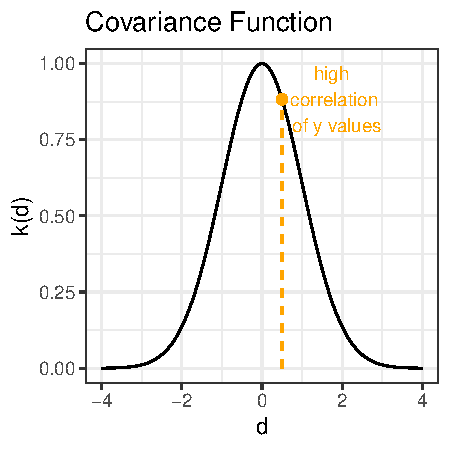
\includegraphics[width=0.45\textwidth]{figure/covariance2point/example_covariance_1.pdf}
      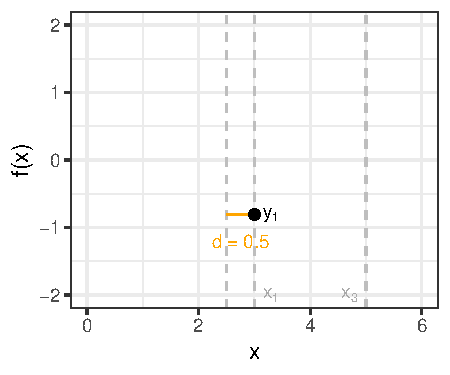
\includegraphics[width=0.45\textwidth]{figure/covariance2point/example_function_1_1.pdf}
    \end{figure}
\end{itemize}

\end{frame}

\begin{vbframe}{Covariance Function of a GP: Example} 

\begin{itemize}
  \item Assume we observed a value $\yi[1] = - 0.8$, the value of $\yi[2]$ should be close under the assumption of the above Gaussian process. 
\end{itemize}

\begin{figure}
  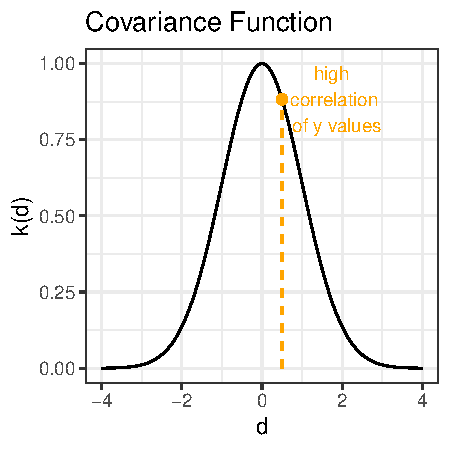
\includegraphics[width=0.45\textwidth]{figure/covariance2point/example_covariance_1.pdf} ~      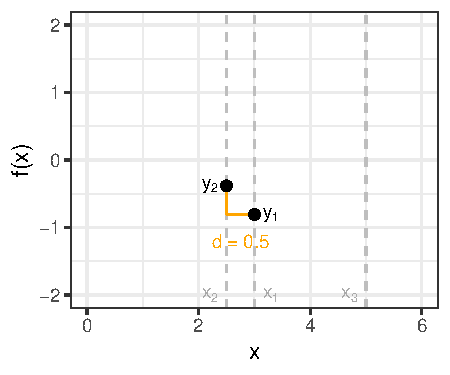
\includegraphics[width=0.45\textwidth]{figure/covariance2point/example_function_1_2.pdf}
\end{figure}

\end{vbframe}


\begin{vbframe}{Covariance Function of a GP: Example} 

\begin{itemize}
  \item Let us compare another point $\xi[3]$ to the point $\xi[1]$
  \item We again compute their correlation
  \item Their function values are not very much correlated; $\yi[1]$ and $\yi[3]$ might be far away from each other
\end{itemize}

\begin{figure}
  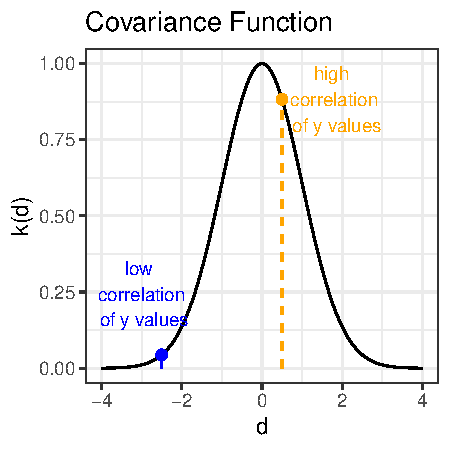
\includegraphics[width=0.45\textwidth]{figure/covariance2point/example_covariance_2.pdf} ~      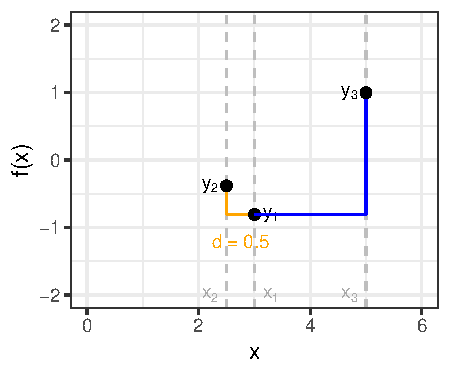
\includegraphics[width=0.45\textwidth]{figure/covariance2point/example_function_2_1.pdf}
\end{figure}

\end{vbframe}

% Given an initial point $\xv^{(1)} = 3$ with $f(\xv^{(1)}) = -0.8$, we want to draw a function value for $\xv^{(2)} = 2.5$. 

% \begin{center}
% \includegraphics{figure_man/covariance2point_1.png}
% \end{center}
% }

% \only<2>{Calculating the distance and using the kernel function as a \enquote{look-up-table} for the correlation of the function values, we see that they are highly correlated. We expect the $y$ values being close.  }

% \only<2>{
% \begin{center}
% \includegraphics{figure_man/covariance2point_2.png}
% \end{center}}

% \only<3->{If in comparison we want to draw a function value for at $x^{(3)} = 5$ given $x^{(1)}$ we see on the right plot that the correlation is low. We do not expect the function value being close to $y^{(1)}$. }

% \only<3>{
% \begin{center}
% \includegraphics{figure_man/covariance2point_3.png}
% \end{center}}

% \only<4>{
% \begin{center}
% \includegraphics{figure_man/covariance2point_4.png}
% \end{center}}



\begin{vbframe}{Covariance Functions}

There are three types of commonly used covariance functions:

\begin{itemize}

\item $k(.,.)$ is called stationary if it is as a function of $\bm{d} = \bm{x} - \bm{x}^\prime$, we write $k(\bm{d})$.\\
Stationarity is invariance to translations in the input space: $k(\bm{x},\bm{x} + \bm{d}) = k(\bm{0}, \bm{d})$
\item $k(.,.)$ is called isotropic if it is a function of $r = \|\bm{x} - \bm{x}^\prime\|$, we write $k(r)$.\\
Isotropy is invariance to rotations of the input space and implies stationarity. 
\item $k(., .)$ is a dot product covariance function if $k$ is a function of $\bm{x}^T \bm{x}^\prime$
\end{itemize}

\end{vbframe}


\begin{vbframe}{Commonly used covariance functions}

\begin{table}[]
\centering
\begin{tabular}{|c|c|}
\hline
Name & $k(\bm{x}, \bm{x}^\prime)$\\
\hline
constant & $\sigma_0^2$ \\ [1em]
linear & $\sigma_0^2 + \bm{x}^T\bm{x}^\prime$ \\ [1em]
polynomial & $(\sigma_0^2 + \bm{x}^T\bm{x}^\prime)^p$ \\ [1em]
squared exponential & $\exp(- \frac{\|\bm{x} - \bm{x}^\prime\|^2}{2\ls^2})$ \\ [1em]
Matérn & \begin{footnotesize} $\frac{1}{2^\nu \Gamma(\nu)}\biggl(\frac{\sqrt{2 \nu}}{\ls}\|\bm{x} - \bm{x}^\prime\|\biggr)^{\nu} K_\nu\biggl(\frac{\sqrt{2 \nu}}{\ls}\|\bm{x} - \bm{x}^\prime\|\biggr)$\end{footnotesize}  \\ [1em]
exponential & $\exp\left(- \frac{\|\bm{x} - \bm{x}^\prime\|}{\ls}\right)$ \\ [1em]
\hline
\end{tabular}
\end{table}
\begin{footnotesize}
$K_\nu(\cdot)$ is the modified Bessel function of the second kind.
\end{footnotesize}


\begin{center}

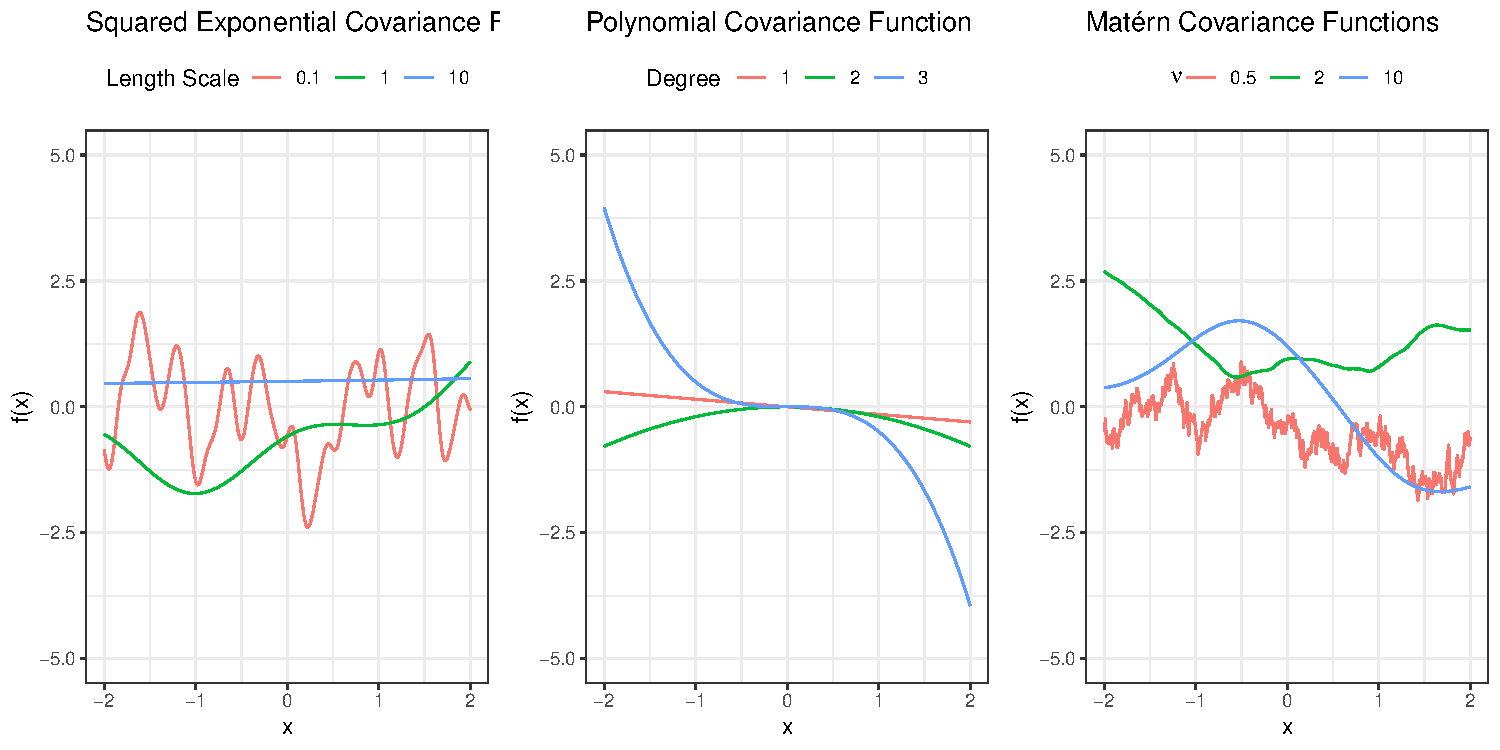
\includegraphics{figure/covariance.pdf}
\end{center}
\vskip -1 em
\begin{footnotesize}
\begin{itemize}
\item Random functions drawn from Gaussian processes with a Squared Exponential Kernel (left), Polynomial Kernel (middle), and a Matérn Kernel (right, $\ls = 1$). 
\item The length-scale hyperparameter determines the ``wiggliness'' of the function.
\item For Matérn, the $\nu$ parameter determines how differentiable the process is.
\end{itemize}
\end{footnotesize}
\end{vbframe}

% \begin{vbframe}{Making New Kernels from Old}

% Kernels can be

% \begin{itemize}
% \item Summed together
% \begin{itemize}
% \item on the same space $k(\xv, \xv') = k_1(\xv, \xv') + k_2(\xv, \xv')$
% \item on tensor space $k(\xv, \xv') = k_1(x_1, x_1') + k_2(x_2, x_2')$
% \end{itemize}
% \item Multiplied together
% \begin{itemize}
% \item on the same space $k(\xv, \xv') = k_1(\xv, \xv') \cdot k_2(\xv, \xv')$
% \item on tensor space $k(\xv, \xv') = k_1(x_1, x_1') \cdot k_2(x_2, x_2')$
% \end{itemize}
% \item Composed with a function $k(\xv, \xv') = k_1(g(\xv), g(\xv'))$ 
% \end{itemize}

% All these operations will preserve the positive definiteness (see exercise). 
% More details: lecture about kernel methods.

% \end{vbframe}
%-----------------------------------------------------------------------

\begin{vbframe}{Squared Exponential Covariance Function}

The squared exponential function is one of the most commonly used covariance functions.
$$
k(\xv, \xv^\prime) = \exp\biggl(- \frac{\|\xv - \xv^\prime\|^2}{2\ls^2}\biggr).
$$

\textbf{Properties}:
\begin{itemize}
\item It depends merely on the distance $r = \|\xv - \xv^\prime\|$ $\to$ isotropic and stationary.\lz
\item Infinitely differentiable $\to$ sometimes deemed 
  unrealistic for modeling most of the physical processes.

\end{itemize}

\end{vbframe}

%%%%%%%%%%%%%%%%%%%%%%%%%%%%%%%%%%%%%%%%%%%%%%%%%%%%%%%%%%%%%%%%%%%%%%%%%%%%%%%%%%%%
\begin{frame}[c,allowframebreaks]{Characteristic Length-Scale}
    $$k(\xv, \xv^\prime) = \exp\left(-\frac{1}{2\ls^2}\|\xv - \xv^\prime\|^2\right)$$
% \begin{figure}
	% \includegraphics[width = .8\textwidth]{figure/lengthscale-1.pdf}
% \end{figure}
$\ls$ is called \textbf{characteristic length-scale}. Loosely speaking, the characteristic length-scale describes how far you need to move in input space for the function values to become uncorrelated. Higher $\ls$ induces smoother functions, lower $\ls$ induces more wiggly functions.

\begin{figure}
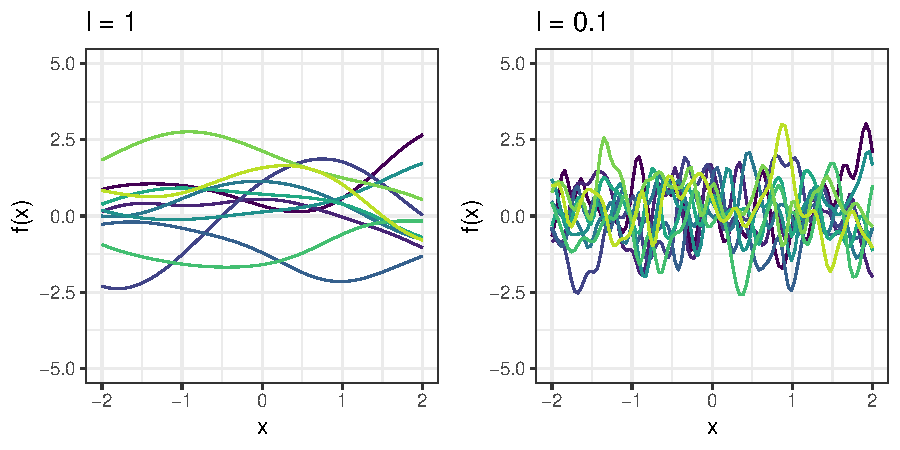
\includegraphics[width=0.6\textwidth]{figure/gp_sample/varying_length_scale.pdf}
\end{figure}

% \begin{itemize}
    % \item Left: for higher $\ls$ the correlation between function values (for unchanged distance of input points) is also higher
    % \item Right plot: a higher $\ls$ induces a smoother function 
% \end{itemize}

\framebreak

For $p \geq 2$ dimensions, the squared exponential can be parameterized:

$$
k(\xv, \xv^\prime) = \exp\,\biggl(- \frac{1}{2}\left(\xv - \xv^\prime\right)^\top\bm{M}\left(\xv - \xv^\prime \right)\biggr)
$$

Possible choices for the matrix $\bm{M}$ include

$$
\bm{M}_1 = \ls^{-2}\id \qquad \bm{M}_2 = \text{diag}(\bm{\ls})^{-2} \qquad \bm{M}_3 = \Gamma \Gamma^\top + \text{diag}(\bm{\ls})^{-2}
$$

where $\bm{\ls}$ is a $p$-vector of positive values and $\Gamma$ is a $p \times k$ matrix. 

\lz

The 2nd (and most important) case can also be written as 
$$
  k(\bold{d}) = \exp\,\biggl(- \frac{1}{2} \sumjp \frac{d_j^2}{l_j^2} \biggr)
$$

% Here again, $\bm{\ls} = (\ls_1,\dots, \ls_p)$ are characteristic length-scales for each dimension. 


\framebreak


What is the benefit of having an individual hyperparameter $\ls_i$ for each dimension?

\vspace{4mm}

\begin{itemize} 
\item The $\ls_1,\dots, \ls_p$ hyperparameters play the role of \textbf{characteristic length-scales}.
\vspace{2mm}
\item Loosely speaking, $\ls_i$ describes how far you need to move along axis $i$ in input space for the function values to be uncorrelated.
\vspace{2mm}
\item Such a covariance function implements \textbf{automatic relevance determination} (ARD), since the inverse of the length-scale $\ls_i$ determines the relevancy of input feature $i$ to the regression.
\vspace{2mm}
\item If $\ls_i$ is very large, the covariance will become almost independent of that input, effectively removing it from inference.
\vspace{2mm}
\item If the features are on different scales, the data can be automatically \textbf{rescaled} by estimating $\ls_1,\dots, \ls_p$ 

\end{itemize}



\framebreak


\begin{figure}
	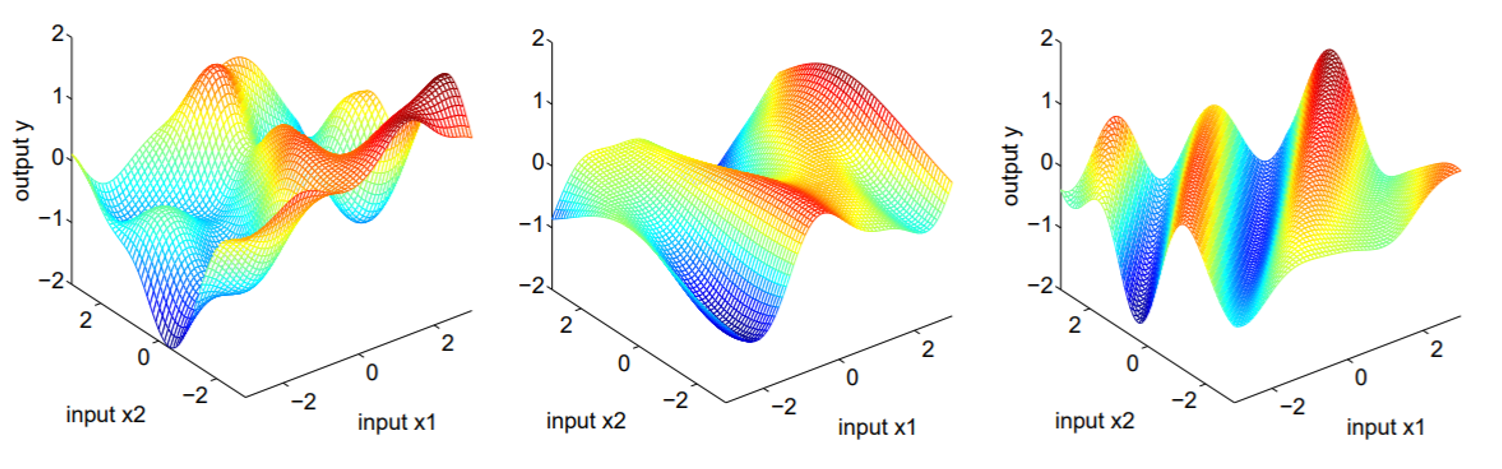
\includegraphics[width = .8\textwidth]{figure_man/covariance2D.png}
\end{figure}

\vspace{3mm}
%\begin{footnotesize}
For the first plot, we have chosen $\bm{M} = \id$: the function varies the same in all directions. The second plot is for $\bm{M} = \text{diag}(\bm{\ls})^{-2}$ and $\bm{\ls} = \left(1, 3 \right)$: The function varies less rapidly as a function of $x_2$ than $x_1$ as the length-scale for $x_1$ is less. In the third plot $\bm{M} = \Gamma \Gamma^T + \text{diag}(\bm{\ls})^{-2}$ for $\Gamma = (1, -1)^\top$ and $\bm{\ls} = (6, 6)^\top$. Here $\Gamma$ gives the direction of the most rapid variation. (Image from Rasmussen \& Williams, 2006)
%\end{footnotesize}


\end{frame}

\endlecture
\end{document}

